\documentclass[10pt]{article}

\usepackage[margin=0.7in]{geometry}
\usepackage{graphicx}
\usepackage{booktabs}
\usepackage{array}
\usepackage{amsmath}
\usepackage{hyperref}
\usepackage{xcolor}
\usepackage{enumitem}
\usepackage{microtype}
\usepackage{tikz}
\usepackage{float}

\usetikzlibrary{arrows.meta, positioning, calc}

\setlength{\parindent}{0pt}
\setlength{\parskip}{4pt}

\setlist[itemize]{
    leftmargin=*,
    topsep=2pt,
    itemsep=1pt,
    parsep=0pt
}

\title{\vspace{-1.5cm}
AI Agent for Dimension Reduction and Exploratory Data Analysis
}

\author{Cassi Chen}
\date{}

\begin{document}

\maketitle
\vspace{-0.7cm}


\section{Introduction and Overview of System Architecture}

Dimension-reduction (DR) analyses and exploratory data analysis (EDA) require decisions for preprocessing, method selection, hyperparameters, evaluation, and interpretation. Unlike a traditional benchmarking study, this project develops an AI agent that automatically performs DR and EDA with minimal human intervention. Given a dataset, the agent inspects the data, determines appropriate preprocessing, selects DR methods, chooses appropriate hyperparamaters, evaluates the results, performs targeted follow-up, and generates a final analysis report autonomously.

The overall agent design in this project was inspired by the UNC BIOS 774 course lecture 9 slides \cite{bios774slides}. Specifically, the researcher sets objectives, the local code performs deterministic computations and saves metrics and results, and the LLM recovers context and invokes the code and explains the result against the task.

Figure~\ref{fig:architecture}, shows the model architecture. Codex (GPT-6 Astra Light) acts as the reasoning agent. It makes preprocessing and method-selection decisions and interprets outputs. Codex uses \texttt{AGENTS.md} and \texttt{SKILL.md} as its main set of instructions, where \texttt{AGENTS.md} defines the repository-wide workflow while \texttt{SKILL.md} files provide statistical guidance for data inspection, preprocessing, DR methods, and embedding evaluation. Skills explain when methods are appropriate and how to interpret their outputs. Local Python programs provide tools for data inspection, preprocessing, DR, and embedding evaluation. The Python tools support three preprocessing choices: None, feature-wise standardization, and library-size normalization followed by \texttt{log1p} transformation. The available DR tools are Isomap, Kernel PCA, Laplacian Eigenmaps, LLE, MDS, PCA, t-SNE, and UMAP. The agent considers all methods but only selects a subset appropriate for the observed data.  


\begin{figure}[H]
    \centering

    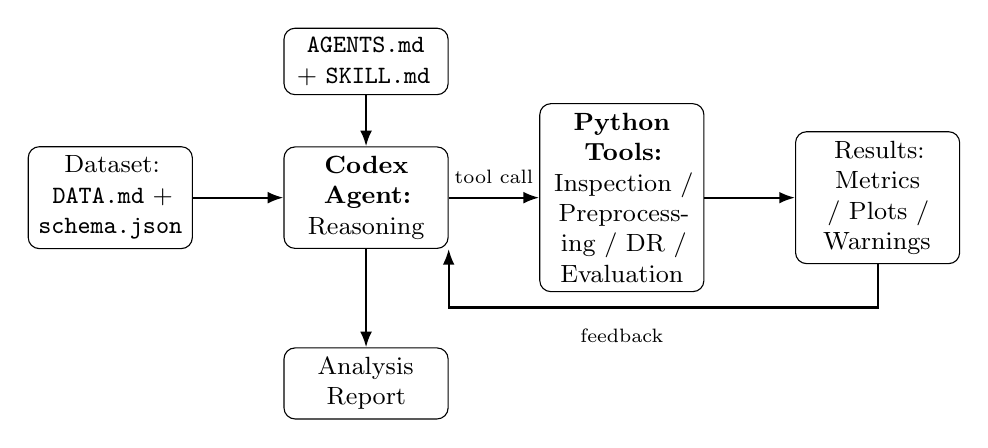
\begin{tikzpicture}[
        node distance=0.65cm and 1.15cm,
        box/.style={
            draw,
            rounded corners,
            align=center,
            minimum height=0.65cm,
            text width=1.85cm,
            font=\small
        },
        arrow/.style={
            -{Latex[length=2mm]},
            thick
        }
    ]

    % Main workflow
    \node[box] (input) {
        Dataset:\\
        \texttt{DATA.md} + \texttt{schema.json}
    };

    \node[box, right=of input] (agent) {
        \textbf{Codex Agent:}\\
        Reasoning
    };

    \node[box, right=of agent] (tools) {
        \textbf{Python Tools:}\\
        Inspection / Preprocessing / DR / Evaluation
    };

    \node[box, right=of tools] (outputs) {
        Results:\\
        Metrics / Plots / Warnings
    };

    % Instructions above
    \node[box, above=0.65cm of agent] (instructions) {
        \texttt{AGENTS.md}\\
        + \texttt{SKILL.md}
    };

    % Report below
    \node[box, below=1.25cm of agent] (report) {
        Analysis Report
    };

    % Main arrows
    \draw[arrow] (input) -- (agent);
    \draw[arrow] (instructions) -- (agent);
    \draw[arrow] (agent) -- (tools);
    \draw[arrow] (tools) -- (outputs);
    \draw[arrow] (agent) -- (report);

    % Tool-call label placed separately
    \node[
        font=\scriptsize,
        above=0.05cm
    ] at ($(agent.east)!0.5!(tools.west)$) {tool call};

    % Feedback loop
    \draw[arrow]
        (outputs.south)
        -- ++(0,-0.55)
        -| (agent.south east);

    % Feedback label placed separately
    \node[
        font=\scriptsize
    ] at ($(tools.south)+(0,-0.55)$) {feedback};

    \end{tikzpicture}

    \caption{Agent architecture.}
    \label{fig:architecture}
\end{figure}


\section{Agent Decision-Making and Implementation}

The agent starts by reading the dataset documentation and invokes the data-inspection tool, which describes dimensions, feature types, missing values, sparsity, and other relevant structural details. 

After preprocessing, the agent considers all the available dimension-reduction methods. Selection of DRs methods is based on the observations from the data inspection skill, method assumptions, computational requirements, and the data structure. 

Broad hyperparameter searches are avoided. Hyperparameters are chosen by the agent, where reasonable default values are provided. If a result appears sensitive to a hyperparameter choice, the agent may perform a small targeted sensitivity analysis. 

If the DR method supports out-of-sample transformation, the models are fitted on the training data and then used to transform evaluation observations. Labels are used afterwards for visualization and interpretation. Note that Kernel PCA, LLE, PCA, Isomap, and UMAP support training and evaluation data. MDS, Laplacian Eigenmaps, and t-SNE support training only.

Embedding evaluation is based on both method-specific and shared diagnostics. For example, PCA reports explained and cumulative variance, while trustworthiness provides a common measure of local-neighborhood preservation.

The main tools and AI models used in this project is provided in Table~\ref{tab:tools}.

\begin{table}[H]
    \centering
    \small
    \setlength{\tabcolsep}{5pt}

    \begin{tabular}{lll}
        \toprule
        \textbf{Component} & \textbf{Type} & \textbf{Role} \\
        \midrule
        Codex (GPT-6 Astra Light) & AI Model & Tool selection, interpretation, reporting \\
        Python scripts & Tools & Inspection, preprocessing, DR, evaluation \\
        \bottomrule
    \end{tabular}

    \caption{Main tools and AI models used in the system.}
    \label{tab:tools}
\end{table}

\section{Experimental Results}

The system was evaluated on two different datasets: PathMNIST \cite{yang2023medmnist} and PBMC3K \cite{pbmc3k}. PathMNIST was evaluated using a class-balanced subset of the original dataset containing 4,500 training images (500 per class) and 900 evaluation images (100 per class). For PBMC3K, 2,638 of the original 2,700 cells had corresponding Seurat cell-type annotations and were retained, with 2,110 cells used for training and 528 for evaluation. Gene filtering and feature selection reduced the PBMC3K dataset to 2,000 genes. Summary of experimental results can be found in Table~\ref{tab:results}.

\begin{table}[H]
    \centering
    \small
    \setlength{\tabcolsep}{4.5pt}
    \begin{tabular}{lcc}
        \toprule
        & \textbf{PathMNIST} & \textbf{PBMC3K} \\
        \midrule
        Preprocessing & None & Log normalize \\
        Selected methods & PCA, UMAP & PCA, UMAP \\
        PCA 2D variance & 57.01\% & 10.12\% \\
        PCA train trustworthiness  & 0.8059 & 0.7891 \\
        PCA eval trustworthiness  & 0.8475 & 0.7892 \\
        UMAP train trustworthiness & 0.8141 & 0.7813 \\
        UMAP eval trustworthiness & 0.8468 & 0.7792 \\
        UMAP Follow-up & $k=30$ & $k=30$ \\
        \bottomrule
    \end{tabular}
    \caption{Summary of results.}
    \label{tab:results}
\end{table}

\textbf{PathMNIST.}

A class-balanced subset of PathMNIST was used. Each $28\times28$ RGB image was represented by 2,352 pixel features; PathMNIST contains flattened histopathology images. Inspection showed that the pixels shared the same intensity scale and had comparable variability. Thus, the agent selected no additional preprocessing.

The first two PCs explained 57.01\% of training variance \ref{fig:pca}(a). PCA and UMAP had similar evaluation trustworthiness (0.8475 and 0.8468, respectively). After observing detached regions in the initial UMAP, the agent performed a targeted follow-up by increasing \texttt{n\_neighbors} from 15 to 30 while holding other hyperparameters fixed. As shown in Figure~\ref{fig:embeddings}(a)--(b), the broad structure remained while smaller geometric details changed, leading the agent to retain the initial hyperparameter settings. Overall, PCA and UMAP reveal broad structure in PathMNIST but substantial overlap among tissue types, suggesting that the dominant sources of variation do not produce clean tissue-class separation in two dimensions

\textbf{PBMC3K.}

In contrast to PathMNIST, PBMC3K inspection showed sparse nonnegative counts and substantial variation in per-cell totals. Thus, the agent selected library-size normalization to 10,000 followed by \texttt{log1p}.



\begin{figure}[H]
    \centering

    % PathMNIST: initial and follow-up
    \begin{minipage}[t]{0.495\linewidth}
        \centering
        
\includegraphics[
            width=\linewidth,
            keepaspectratio
        ]{../outputs/final_dataset_1/umap_train_2d.png}
        \vspace{-2mm}

        \small (a) PathMNIST, $k=15$
    \end{minipage}
    \hspace{-2mm}
    \begin{minipage}[t]{0.495\linewidth}
        \centering
        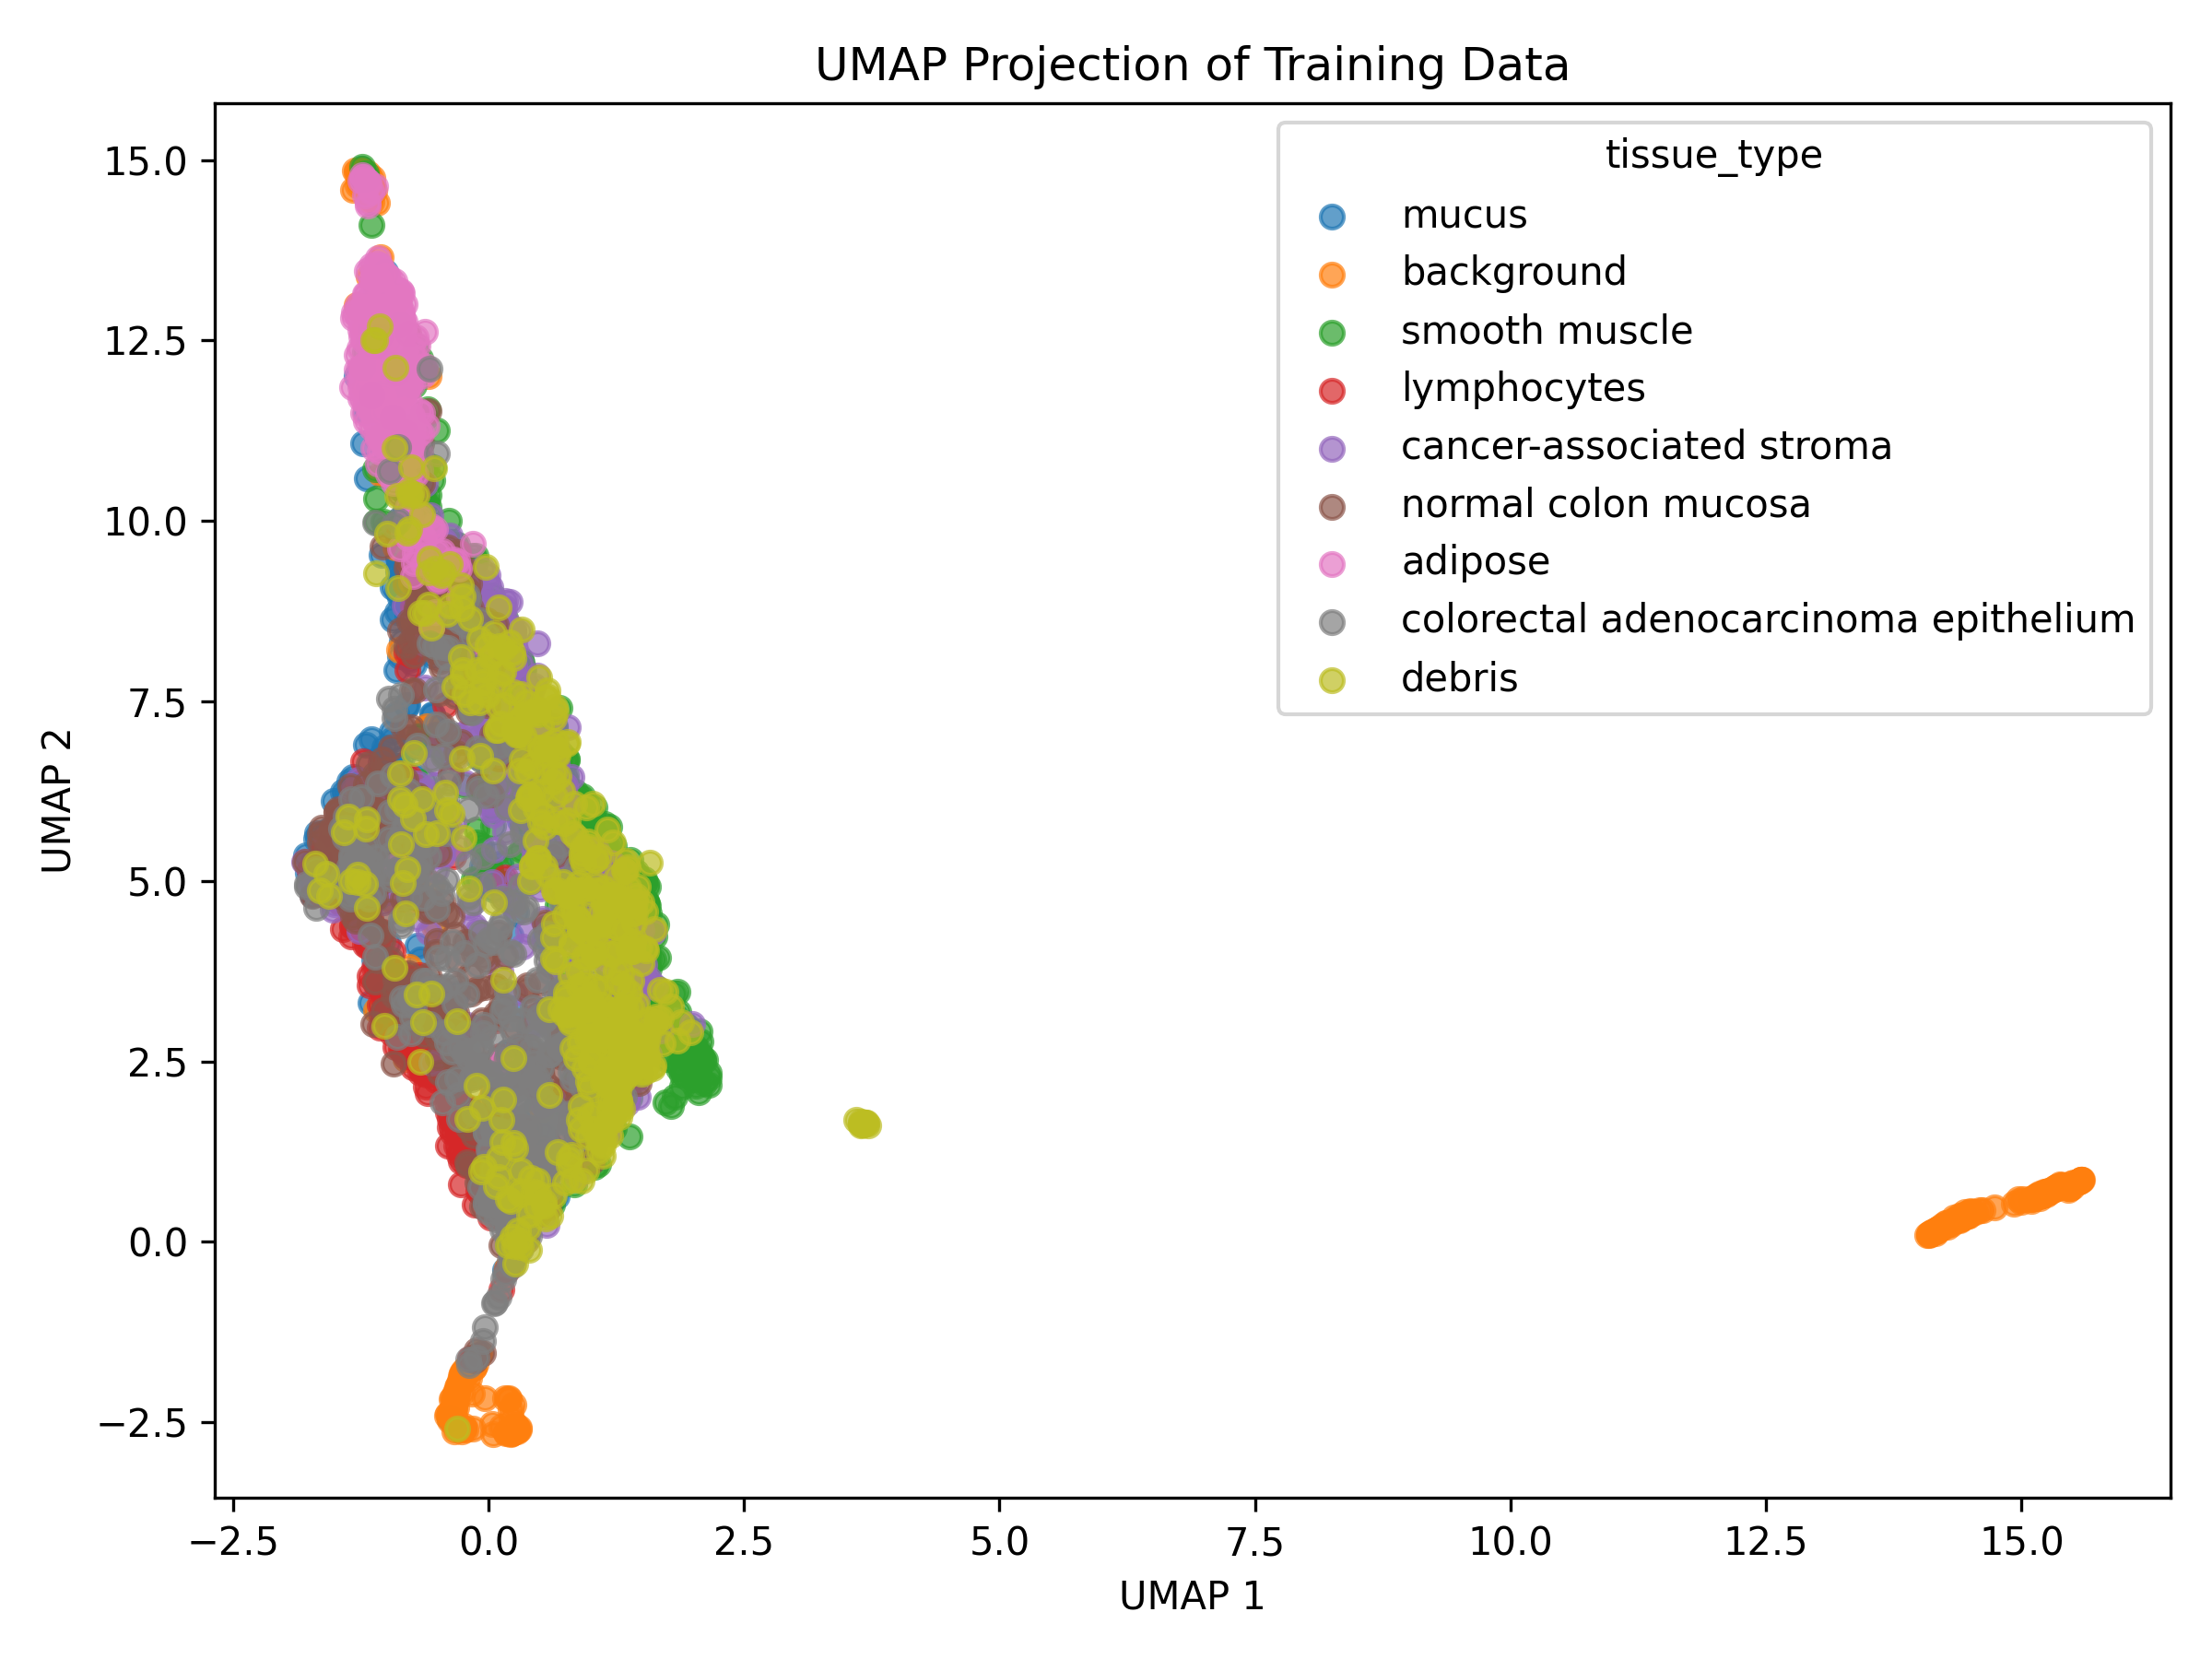
\includegraphics[
            width=\linewidth,
            keepaspectratio
        ]{../outputs/final_dataset_1/followup_neighbors30/umap_train_2d.png}
        \vspace{-2mm}

        \small (b) PathMNIST, $k=30$
    \end{minipage}

    \vspace{1mm}

    % PBMC3K: initial and follow-up
    \begin{minipage}[t]{0.495\linewidth}
        \centering
        
\includegraphics[
            width=\linewidth,
            keepaspectratio
        ]{../outputs/final_dataset_2/umap_train_2d.png}
        \vspace{-2mm}

        \small (c) PBMC3K, $k=15$
    \end{minipage}
    \hspace{-2mm}
    \begin{minipage}[t]{0.495\linewidth}
        \centering
        
\includegraphics[
            width=\linewidth,
            keepaspectratio
        ]{../outputs/final_dataset_2/followup_umap_30/umap_train_2d.png}
        \vspace{-2mm}

        \small (d) PBMC3K, $k=30$
    \end{minipage}

    \vspace{-1mm}

    \caption{UMAP training embeddings before and after the agent's targeted
    sensitivity analysis.}
    \label{fig:embeddings}
\end{figure}

The first two PCs explained only 10.12\% of training variance, meaning that there is substantial information beyond two dimensions \ref{fig:pca}(b). Similarly to PathMNIST, PCA and UMAP had similar evaluation trustworthiness (0.7892 and 0.7792, respectively). Also similarly to PathMNIST, separated UMAP regions prompted the agent to increase \texttt{n\_neighbors} from 15 to 30 while holding other hyperparameters fixed. As shown in Figure~\ref{fig:embeddings}(c)--(d), broad structure remained while relative placement changed. Overall, PCA and UMAP reveal broad cell-type-associated structure in PBMC3K, particularly for monocyte- and B-cell populations. However, there is substantial overlap among other cell types.

\begin{figure}[H]
    \centering

    % PathMNIST PCA
    \begin{minipage}[t]{0.495\linewidth}
        \centering
        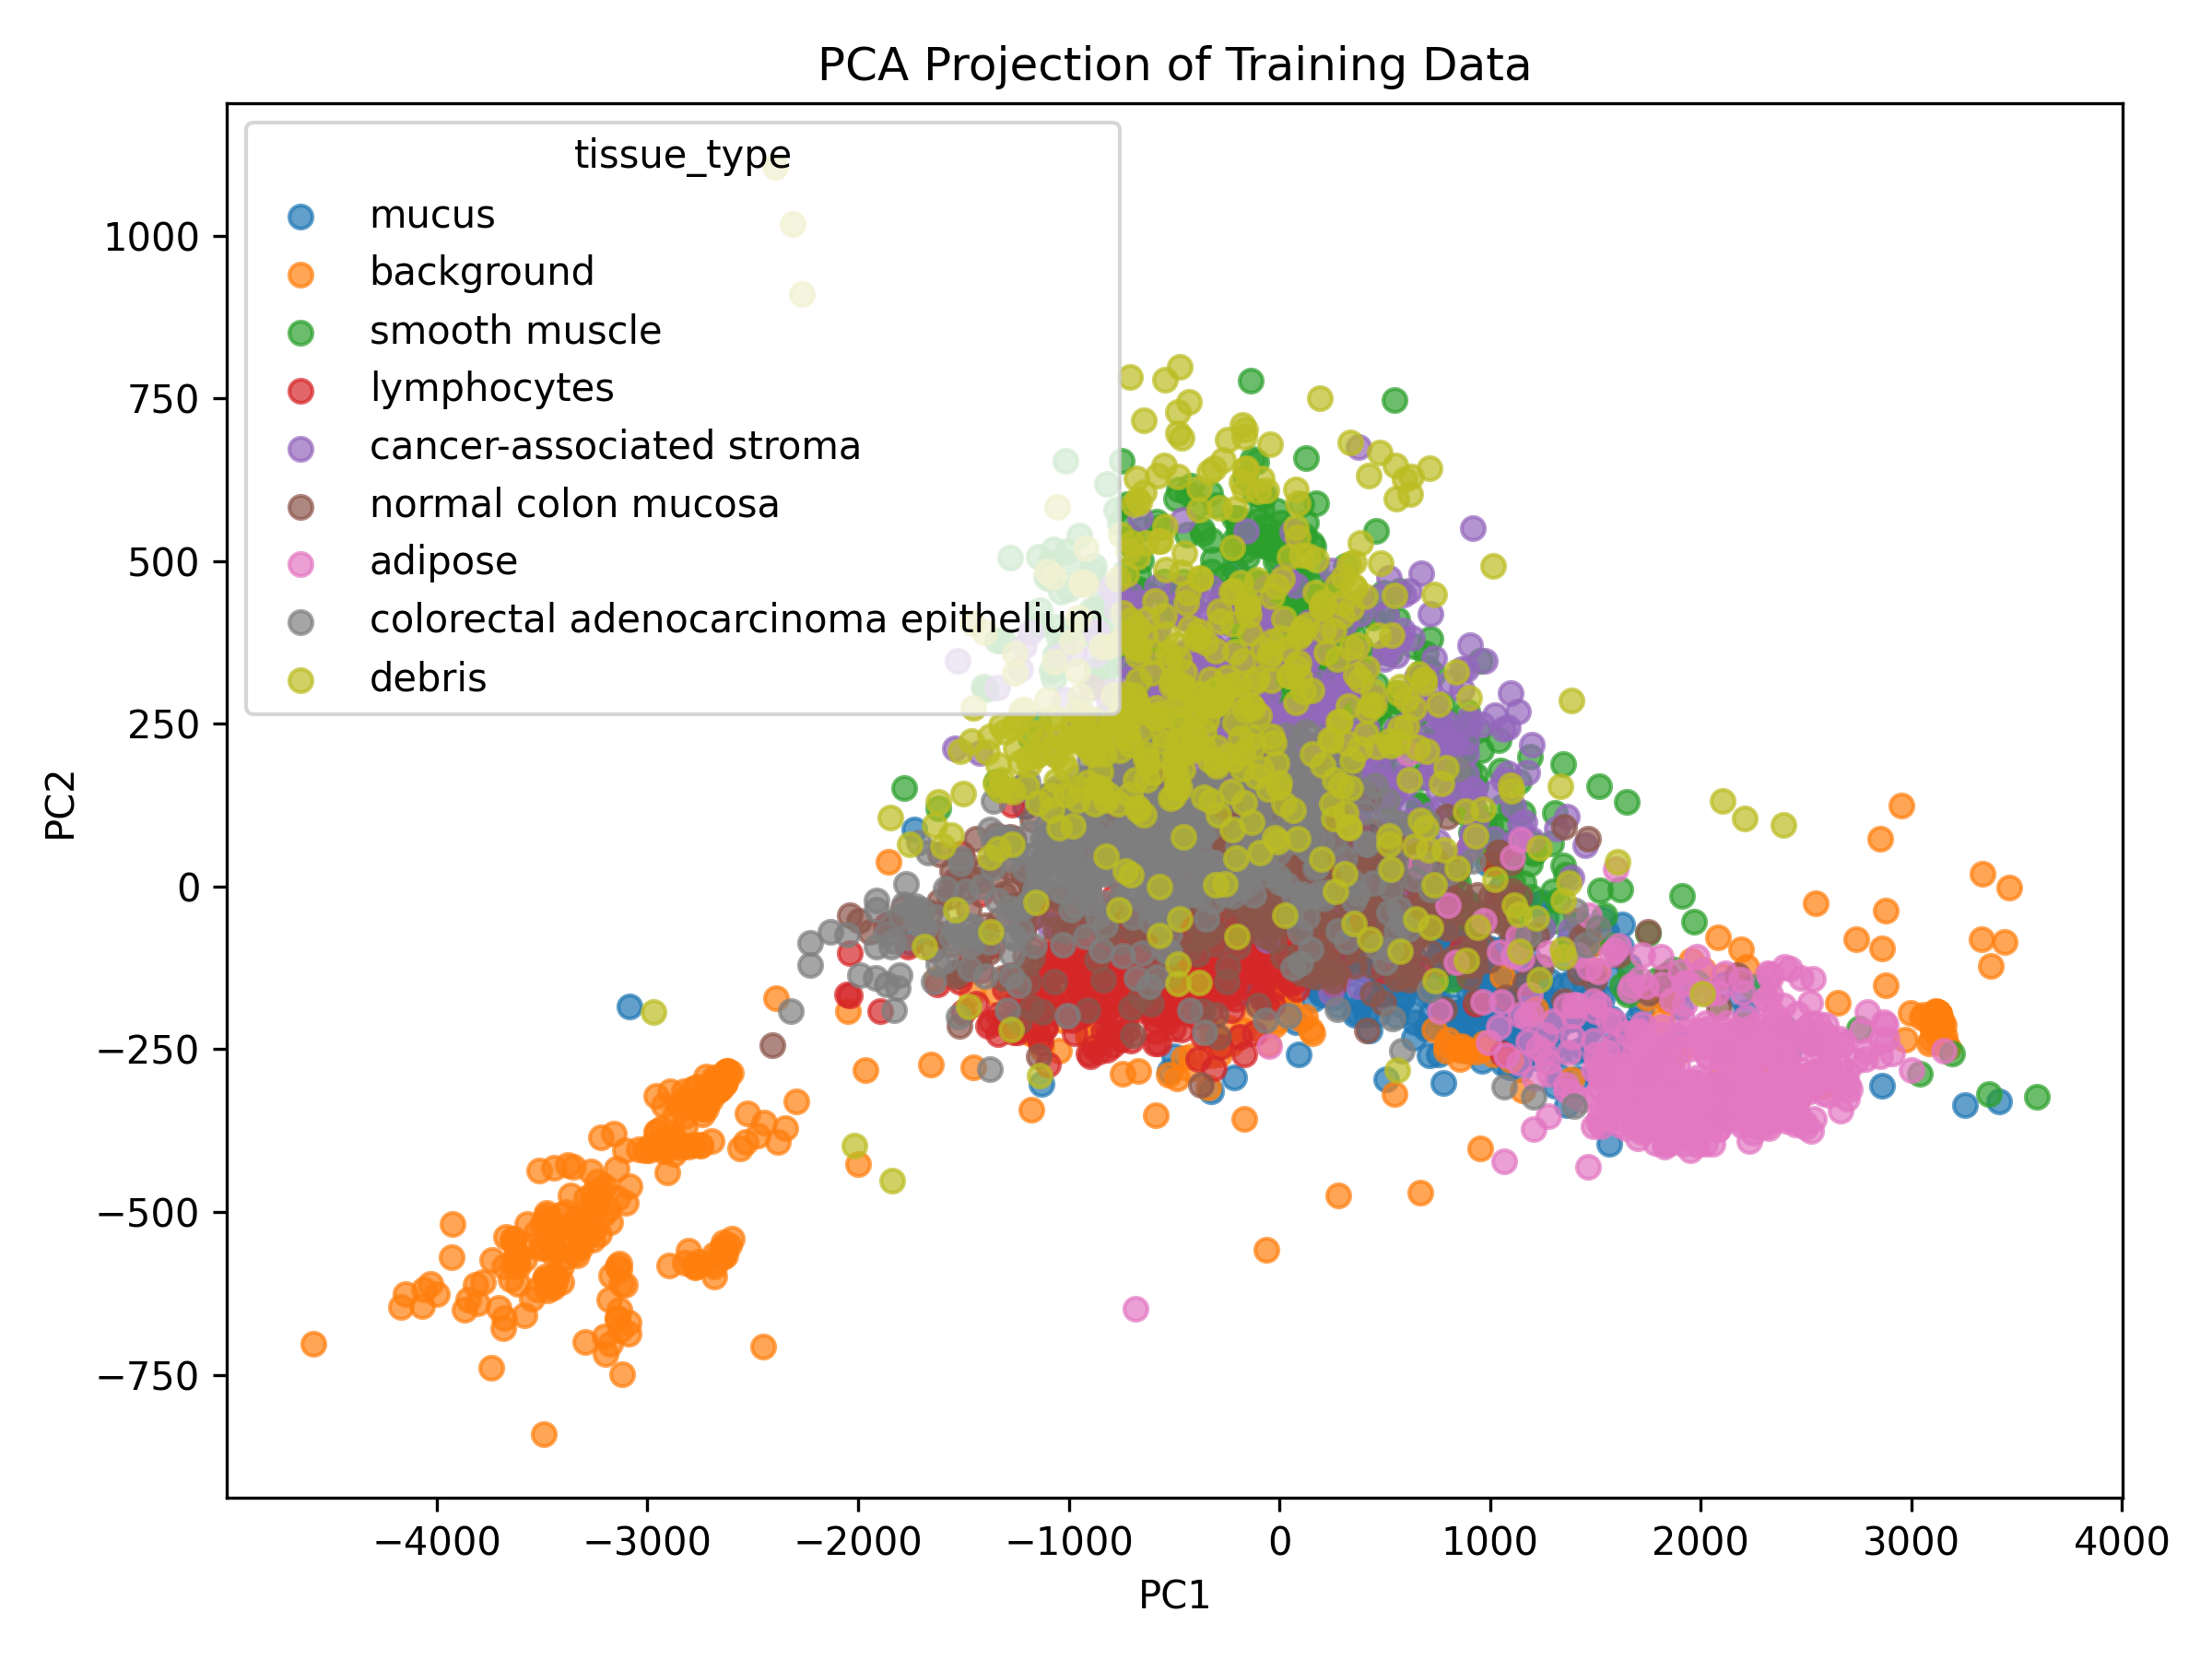
\includegraphics[
            width=\linewidth,
            keepaspectratio
        ]{../outputs/final_dataset_1/pca_train_2d.png}
        \vspace{-2mm}
        \small (a) PathMNIST
    \end{minipage}
    \hspace{-2mm}
    % PBMC3K PCA
    \begin{minipage}[t]{0.495\linewidth}
        \centering
        
\includegraphics[
            width=\linewidth,
            keepaspectratio
        ]{../outputs/final_dataset_2/pca_train_2d.png}
        \vspace{-2mm}
        \small (b) PBMC3K
    \end{minipage}

    \vspace{-1mm}

    \caption{PCA training embeddings.}

    \label{fig:pca}
\end{figure}

\section{Strengths, Limitations, and Conclusion}

The main strength of the system is that entire process, including preprocessing, picking DR methods, choosing hyperparameters, and conducting evaluations, is autonomously done by an agent. The two tests conducted on PathMNIST and PBMC3K shows that the agent is able to adapt across different data modalities. 

The system also has many limitations. First, the agent can only choose among the supplied preprocessing and DR methods. Second, method and hyperparameter selection rely only on LLM reasoning instead of a optimization criterion. Finally, trustworthiness measures only local-neighborhood preservation, while method-specific diagnostics assess distinct properties of the embeddings, making direct comparisons across metrics difficult.

Overall, this project showcases an AI agent that can translate a DR task into an executable task, while maintaining reproducibility.

\begin{thebibliography}{9}

    \bibitem{bios774slides}
    Longfei Zhang.
    BIOS 774 Course Slides.
    \textit{An Intro to Building Agents in 2026},
    2026.

    \bibitem{yang2023medmnist}
    Jiancheng Yang, Rui Shi, and Bingbing Ni.
    MedMNIST v2: A large-scale lightweight benchmark for 2D and 3D biomedical image classification.
    \textit{Scientific Data}, 10:41, 2023.

    \bibitem{pbmc3k}
    10x Genomics.
    \textit{PBMC 3K Dataset}.
    10x Genomics.

    
    \end{thebibliography}

\end{document}